\documentclass[12pt, a4paper]{article}
\usepackage{fontspec}
\usepackage{xeCJK}
\usepackage{hyperref}
\usepackage{enumitem}
\setCJKmainfont{微軟正黑體}
\XeTeXlinebreaklocale "zh"
\XeTeXlinebreakskip = 0pt plus 1pt
\usepackage{enumerate}
\usepackage{graphicx}
\usepackage{array}
\date{}
\title{\vspace{-3.0cm} 計算機結構 \hspace{0cm} Exercise 03 \\ \vspace{0cm}}
\author{\normalsize B03902062 \hspace{0cm} 資工三 \hspace{0cm} 董文捷}
\begin{document}
\maketitle
\begin{itemize}[font=\bfseries]

\item[4.4.1]
critical path = Instruction memory \\
cycle time = $200ps$ 
\item[4.4.2]
\scalebox{0.96}{critical path = Instruction memory + Sign extend + Shift left + Add + Mux} \\
\scalebox{0.96}{cycle time = $200ps$ + $15ps$ + $10ps$ + $70ps$ + $20ps$ = $315ps$}
\item[4.4.3]
\scalebox{0.9}{time to calculate PCsrc = Regs + Mux + ALU = $90ps$ + $20ps$ + $90ps$ = $200ps$} \\
\scalebox{0.88}{time to calculate branch target = Sign extend + Shift left + Add = $15ps$ + $10ps$ + $70ps$ = $95ps$} \\
\scalebox{0.96}{critical path = Instruction memory + Regs + Mux + ALU + Mux} \\
\scalebox{0.96}{cycle time = $200ps$ + $200ps$ + $20ps$ = $420ps$}
\item[4.4.4]
Branch instructions and jumps require Shift-left-2.
\item[4.4.5]
For branch instructions, it takes more time to decide whether to branch or not than calculating the branch target, so Shift-left-2 is not on the critical path. Shift-left-2 is on the critical path of jumps.
\item[4.4.6]
For \texttt{beq} instructions, since Shift-left-2 is not on the critical path, latency is not affected. \texttt{add} instructions take Instruction memory + Regs + Mux + ALU + Mux = $420ps$, which is not affected either. The only case that latency of Shift-left-2 will affect the cycle time is Shift-left-2 > $115ps$, then it is on the critical path of \texttt{beq}, and \texttt{beq} will take more time than \texttt{add}, making the cycle time longer. Since Shift-left-2 is usually quite effective, this case is almost impossible.

\item[4.8.1]
clock cycle time in a non-pipelined processor \\ = $250ps$ + $350ps$ + $150ps$ + $300ps$ + $200ps$ = $1250ps$ \\
clock cycle time in a pipelined processor \\ = maximum latency for an individual stage = $350ps$
\item[4.8.2]
total latency in a non-pipelined processor \\ = IF + ID + EX + MEM + WB = $1250ps$ \\
total latency in a pipelined processor \\ = total latency in a non-pipelined processor \\ = $1250ps$ (Latency for each instruction not reduced) 
\item[4.8.3]
Since clock cycle in a pipelined processor is decided by the maximum latency for an individual stage, we should split ID into two stages, each with latency of $175ps$. The new clock cycle time is then decided by MEM, which is $300ps$.
\item[4.8.4]
utilization of the data memory = lw + sw = $35\%$
\item[4.8.5]
utilization of the write-register port = alu + lw = $65\%$
\item[4.8.6]
clock cycle time \\
single-cycle : $1250ps$ \\
multi-cycle : maximum latency for an individual stage = $350ps$ \\
pipelined : $350ps$ \\
\vspace*{-0.4cm} \\
$\longrightarrow$ single-cycle > multi-cycle = pipelined \\
\vspace*{-0.3cm} \\
execution time \\
single-cycle : \\
$1250ps \times 100\% = 1250ps$ \\
multi-cycle : \\
alu = IF + ID + EX + WB = 4 cycles = $1400ps$ \\
beq = IF + ID + EX = 3 cycles = $1050ps$ \\
lw = IF + ID + EX + MEM + WB = 5 cycles = $1750ps$ \\
sw = IF + ID + EX + MEM = 4 cycles = $1400ps$ \\
$1400ps \times 45\% + 1050ps \times 20\% + 1750ps \times 20\% + 1400ps \times 15\% = 1400ps$ \\
pipelined : \\
$350ps \times 100\% = 350ps$ \\
\vspace*{-0.4cm} \\
$\longrightarrow$ multi-cycle > single-cycle > pipelined \\

\item[4.9.1]
According to \href{https://en.wikipedia.org/wiki/Data_dependency}{Data dependency}, there are three types of data dependences, anti-dependence, flow dependence, and output dependence. \\
\scalebox{0.92}{Between \texttt{or r1, r2, r3} and \texttt{or r2, r1, r4} : anti-dependence + flow dependence} \\
\scalebox{0.92}{Between \texttt{or r2, r1, r4} and \texttt{or r1, r1, r2} : anti-dependence + flow dependence} \\
\scalebox{0.92}{Between \texttt{or r1, r2, r3} and \texttt{or r1, r1, r2} : output dependence} 
\item[4.9.2] If there is no forwarding \\ 
Data hazard between \texttt{or r1, r2, r3} and \texttt{or r2, r1, r4} : \\ To wait result of \texttt{r1}, ID of second instruction can not be executed earlier than WB of first instruction $\rightarrow$ 2 bubbles \\
Data hazard between \texttt{or r2, r1, r4} and \texttt{or r1, r1, r2} : \\ To wait result of \texttt{r2} $\rightarrow$ 2 bubbles \\
\newpage
\texttt{or r1, r2, r3} \\
\texttt{nop} \\
\texttt{nop} \\
\texttt{or r2, r1, r4} \\
\texttt{nop} \\
\texttt{nop} \\
\texttt{or r1, r1, r2} \\
\item[4.9.3]
All hazards are eliminated by forwarding the result of EX stage to next instruction. \\
\texttt{or r1, r2, r3} \\
\texttt{or r2, r1, r4} \\
\texttt{or r1, r1, r2} \\
\item[4.9.4]
Without Forwarding : $250ps \times (5 + 2 + 1 + 2 + 1) = 2750ps$ \\
With Full Forwarding : $300ps \times (5 + 1 + 1) = 2100ps$ \\
Speedup = $\displaystyle \frac{2750ps}{2100ps} = 1.31$ 
\item[4.9.5]
To eliminate hazards, forwarding from the MEM to the EX stage is not needed because all instructions are ALU instructions. \\
\texttt{or r1, r2, r3} \\
\texttt{or r2, r1, r4} \\
\texttt{or r1, r1, r2} \\
\item[4.9.6]
Without Forwarding : $250ps \times (5 + 2 + 1 + 2 + 1) = 2750ps$ \\
With ALU-ALU Forwarding Only: $290ps \times (5 + 1 + 1) = 2030ps$ \\
Speedup = $\displaystyle \frac{2750ps}{2030ps} = 1.35$ 

\newpage
\item[4.11.1]
\hspace*{0cm} \\
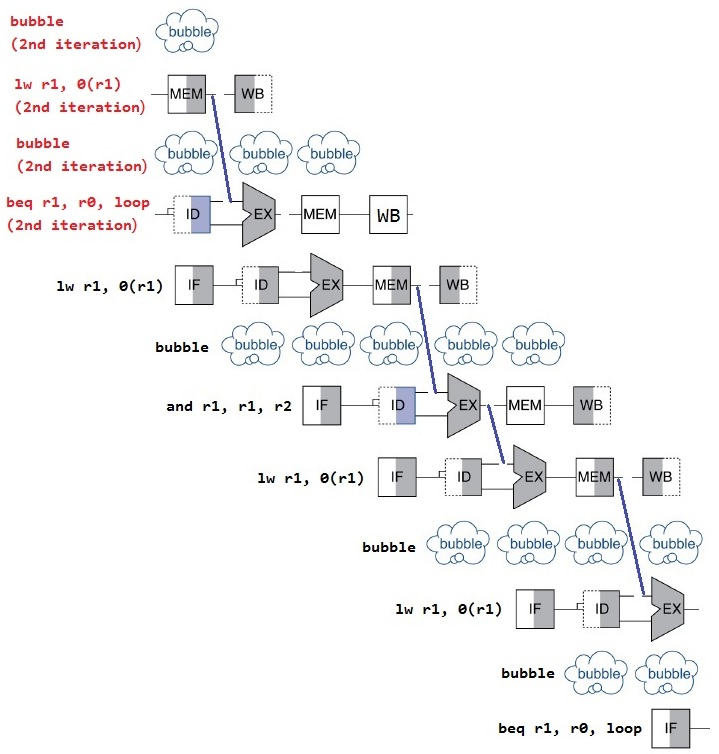
\includegraphics[scale = 0.75]{3_2.JPG}
\item[4.11.2]
According to the above figure, it takes 8 cycles for each iteration of the loop, but the situation that all five pipeline stages are doing useful work never happens because there are always some bubbles in one or two stages. $\displaystyle \frac{0}{8} = 0\%$.

\newpage
\item[4.13.1]
\texttt{add r5, r2, r1} \\
\texttt{nop} \\
\texttt{nop} \\
\texttt{lw r3, 4(r5)} \\
\texttt{lw r2, 0(r2)} \\
\texttt{nop} \\
\texttt{or r3, r5, r3} \\
\texttt{nop} \\
\texttt{nop} \\
\texttt{sw r3, 0(r5)} \\
\item[4.13.2]
The only instruction that can be rearranged is \texttt{lw r2, 0(r2)}, but it does not cause any hazard. Orders of other instructions can not be changed because of their flow dependences. Therefore, no hazard can be avoided. \\
\texttt{add r5, r2, r1} \\
\texttt{nop} \\
\texttt{nop} \\
\texttt{lw r3, 4(r5)} \\
\texttt{lw r2, 0(r2)} \\
\texttt{nop} \\
\texttt{or r3, r5, r3} \\
\texttt{nop} \\
\texttt{nop} \\
\texttt{sw r3, 0(r5)} \\
\item[4.13.3]
If there is forwarding, all hazards are eliminated. Even without hazard detection unit, this code can still execute correctly.  
\item[4.13.4]
Since there are no bubbles, \texttt{PCWrite} and \texttt{IF/IDWrite} is always 1, and \texttt{ID/EXZero} is always 0. For EX hazard, \texttt{ForwardA} or \texttt{ForwardB} will be \texttt{10}. For MEM hazard, \texttt{ForwardA} or \texttt{ForwardB} will be \texttt{01}. \texttt{ForwardA} and \texttt{ForwardB} of the first two cycles are unknown because we do not know whether forwarding from previous instructions is needed. \\
\newpage
\scalebox{0.9}{\texttt{PCWrite} = 1, \texttt{IF/IDWrite} = 1, \texttt{ID/EXZero} = 0, \texttt{ForwardA} and \texttt{ForwardB} are unknown.} \\
\scalebox{0.9}{\texttt{PCWrite} = 1, \texttt{IF/IDWrite} = 1, \texttt{ID/EXZero} = 0, \texttt{ForwardA} and \texttt{ForwardB} are unknown.} \\
\scalebox{0.9}{\texttt{PCWrite} = 1, \texttt{IF/IDWrite} = 1, \texttt{ID/EXZero} = 0, \texttt{ForwardA} = \texttt{00}, \texttt{ForwardB} = \texttt{00}.} \\
\scalebox{0.9}{\texttt{PCWrite} = 1, \texttt{IF/IDWrite} = 1, \texttt{ID/EXZero} = 0, \texttt{ForwardA} = \texttt{01}, \texttt{ForwardB} = \texttt{00}.} \\ (\texttt{lw r3, 4(r5)} forwarding \texttt{r5} from \texttt{add r5, r2, r1}) \\
\scalebox{0.9}{\texttt{PCWrite} = 1, \texttt{IF/IDWrite} = 1, \texttt{ID/EXZero} = 0, \texttt{ForwardA} = \texttt{00}, \texttt{ForwardB} = \texttt{00}.} \\
\item[4.13.5] 
If there is no forwarding, we have to check whether \texttt{EX/MEM.RegisterRd} or \texttt{MEM/WB.RegisterRd} is the same as \texttt{ID/EX.RegisterRs} or \texttt{ID/EX.RegisterRt} in Hazard detection unit, just like Forwarding unit does. Every forwarding requirement results in a hazard. \texttt{PCWrite}, \texttt{IF/IDWrite}, and \texttt{ID/EXZero} of Hazard detection unit are already able to handle bubbles, no extra output signals are needed.
\item[4.13.6]
\texttt{PCWrite} = 1, \texttt{IF/IDWrite} = 1, \texttt{ID/EXZero} = 0 \\
\texttt{PCWrite} = 1, \texttt{IF/IDWrite} = 1, \texttt{ID/EXZero} = 0 \\
\texttt{PCWrite} = 1, \texttt{IF/IDWrite} = 1, \texttt{ID/EXZero} = 0 \\
\texttt{PCWrite} = 0, \texttt{IF/IDWrite} = 0, \texttt{ID/EXZero} = 1 \\
\texttt{PCWrite} = 0, \texttt{IF/IDWrite} = 0, \texttt{ID/EXZero} = 1 \\
(2 bubbles $\rightarrow$ \texttt{r5} is still not ready)
\item[4.16.1]
accuracy of always-taken predictors = $\displaystyle \frac{3}{5} = 60\%$ \\
accuracy of always-not-taken predictors = $\displaystyle \frac{2}{5} = 40\%$ 
\item[4.16.2]
\begin{enumerate}[(1)]
\item Predict NT, state transits to the bottom right state.
\item Predict NT, state transits to the bottom left state.
\item Predict NT, state transits to the bottom right state.
\item Predict NT, state transits to the top right state.
\end{enumerate}
accuracy = $\displaystyle \frac{1}{4} = 25\%$ 
\newpage
\item[4.16.3]
If this pattern is repeated forever, the predictor will start off in the top right state in every loop, and then
\begin{enumerate}[(1)]
\item Predict T, state transits to the top left state.
\item Predict T, state transits to the top right state.
\item Predict T, state transits to the top left state.
\item Predict T, state remains unchanged.
\item Predict T, state goes back to the top right state.
\end{enumerate}
accuracy = $\displaystyle \frac{3}{5} = 60\%$ 

\end{itemize}
\end{document}